We begin by using Karma's existing capability to capture the artists in the first CSV file as crm:E21\_Person from the CIDOC CRM ontology in a source model shown in Figure~\ref{fig:simple-model-screenshot}.  
Karma can translate this model into an R2RML mapping.
Karma can then compare it to the other mappings loaded in the Model Manager to discover new ways to integrate data.


\begin{figure*}
\begin{center}
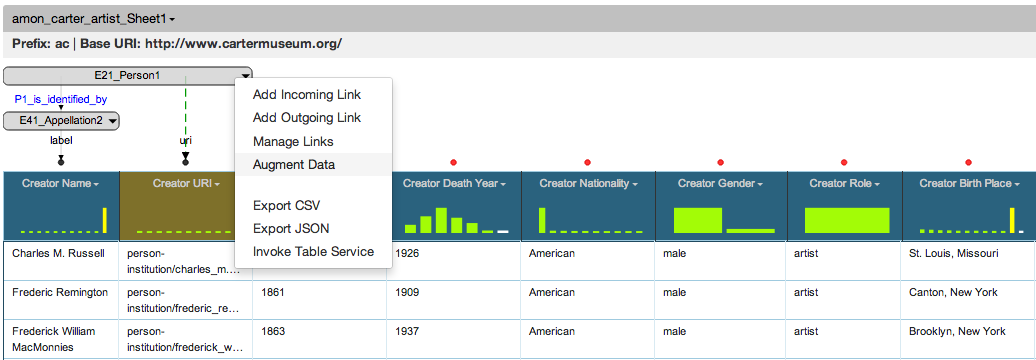
\includegraphics[width=4.8in]{images/4-simple-model.png}
\vspace{-3mm}
\caption{A Karma user has created an R2RML mapping for a CSV file of a museum's artists' biographical records and attempts to discover new data to augment the records}
\vspace{-2mm}
\label{fig:simple-model-screenshot}
\end{center}
\vspace{-1.5em}
\end{figure*}
